\clearpage{\pagestyle{empty}\cleardoublepage}
\chapter{Contesto}
\lhead[\fancyplain{}{\bfseries\thepage}]{\fancyplain{}{\bfseries\rightmark}}
\pagenumbering{arabic}

TODO: descrizione di una pagina sugli argomenti che andremo a trattare in questo capitolo \newpage

\section{Open Data} % : definizione e contesto
Le nuove tecnologie permettono di creare servizi in grado di migliorare la vita dei cittadini e di far funzionare più efficientemente governi e società. Molti dei dati necessari a raggiungere questi obiettivi sono prodotti da organismi pubblici, tuttavia spesso tali dati non sono disponibili in formati che li rendano facili da manipolare.
Per questo motivo, da diversi anni si utilizza la nozione di dati aperti, i cosiddetti \textit{open data}, e più specificamente i dati aperti del settore pubblico, intesi come informazione, pubblica o privata, accessibile e riutilizzabile da chiunque e per qualsiasi fine. L'uso comune del termine inizia nel 2009, quando diversi governi hanno annunciato nuove iniziative per l'apertura della loro informazione pubblica, tra cui quelli di Stati Uniti, Regno Unito, Canada e Nuova Zelanda.

\begin{figure}[H]
    \centering
    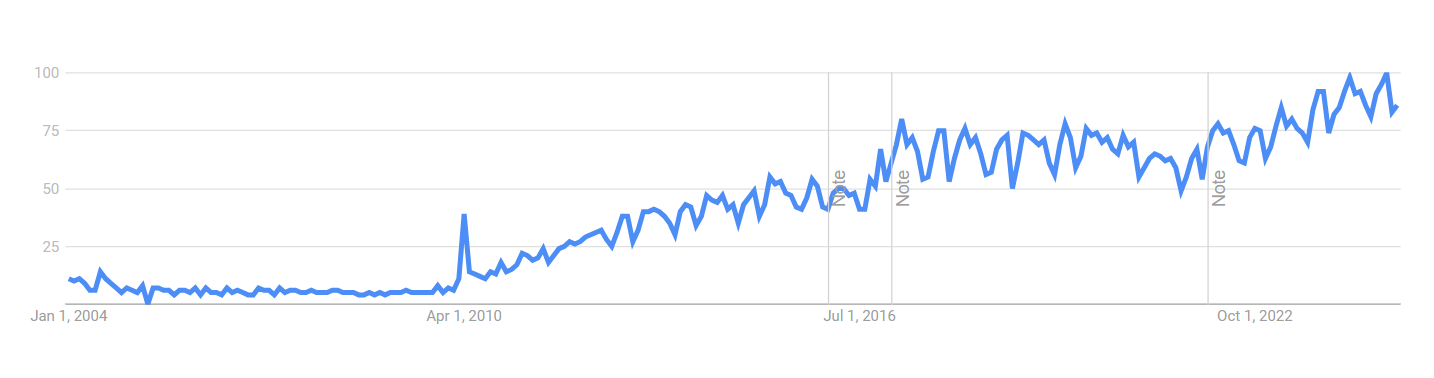
\includegraphics[width=\textwidth]{open_data_google_trends}
    \caption[Open Data su Google Trends]{Ricerche su Google collegate al termine Open Data, effettuate tra il 2004 e il 2025. Notare l'aumento successivo al 2009 e il trend in crescita.}
\end{figure}

\subsection{Concetto di Open Data}
%Definizione e principi fondamentali


\subsection{Caratteristiche principali degli Open Data}
Accessibilità, Interoperabilità, Riutilizzabilità

Formati comuni: CSV, JSON, XML

\subsection{Confronto con dati privati}
Differenze principali

Vantaggi e svantaggi rispetto agli Open Data

\subsection{Contesto italiano e internazionale}
\subsubsection{Iniziative globali}
Open Government Partnership

\subsubsection{Normativa italiana}
CAD (Codice dell'Amministrazione Digitale)

\subsubsection{Portali di Open Data}
dati.gov.it

Open Data Bologna (https://opendata.comune.bologna.it/)

\subsubsection{Casi studio e iniziative significative}
INSPIRE

Copernicus


\section{Bologna e progetto BolognaWiFi}  %  e Comune di Bologna
\subsection{Bologna Smart City}
\subsubsection{Digitalizzazione e innovazione urbana}
Progetti principali

\subsubsection{Politiche locali per gli Open Data}
Strategie e risultati

\subsubsection{Infrastrutture digitali recenti}
Implementazioni chiave

\subsection{Progetto BolognaWiFi}
\subsubsection{Obiettivi principali}
Scopi e finalità del progetto

\subsubsection{Tipologie di dati raccolti}
Flussi utenti

Accessi WiFi

Affluenza in aree urbane

\subsubsection{Statistiche recenti}
Dati sull'uso del WiFi pubblico a Bologna

\subsubsection{Risorse utili}
Documentazione ufficiale del progetto

Report e analisi pubblicati dal Comune


\section{Visualizzazione dei dati}  % Analisi e
\subsection{Importanza della visualizzazione}
\subsubsection{Analisi dei dati urbani}
Esempi pratici e benefici

\subsubsection{Supporto decisionale}
Impatti sulle amministrazioni pubbliche

\subsection{Caratteristiche di una buona visualizzazione}
Chiarezza e semplicità

Interattività e Accessibilità

\subsection{Strumenti di visualizzazione}
\subsubsection{Panoramica degli strumenti comuni}
Tableau

D3.js

\subsubsection{Vantaggi e svantaggi degli strumenti}
Breve descrizione comparativa

\subsubsection{Applicazioni pratiche}
Esempi nelle smart cities


\section{Sfide e opportunità}   % Benefici e potenziale degli Open Data
\subsection{Sfide tecniche}
\subsubsection{Gestione di dataset eterogenei}
Problemi e soluzioni

\subsubsection{Scalabilità e performance}
Tecnologie per ottimizzare

\subsection{Aspetti etici e legali}
\subsubsection{Privacy e anonimizzazione dei dati}
Strumenti e tecniche utilizzate

\subsubsection{Licenze e diritti d'uso}
Regolamenti e pratiche comuni

\subsubsection{Casi noti di violazioni}
Esempi significativi e lezioni apprese

\subsection{Opportunità}
\subsubsection{Trasparenza e coinvolgimento}
Benefici per cittadini e istituzioni

\subsubsection{Pianificazione urbana}
Utilizzo dei dati per migliorare i servizi

\subsubsection{Collaborazioni pubblico-privato}
Partnership per sfruttare al meglio gli Open Data

\subsection{Fonti per approfondire}
\subsubsection{Linee guida GDPR}
Applicazioni rilevanti per i dati urbani

\subsubsection{Studi accademici}
Temi su etica e Open Data